
\section{Eclipse (Git, Maven plug-ins integrated)}

If you have an Eclipse IDE for Java Developers with version $\ge$ 3.7, you could probably skip this task. But if you are stuck in a situation where you were told Eclipse is missing a plug-in, you might want to return to this section. If you have other packages (Eclipse Classic or Eclipse for Java EE Developers), please do not skip this task.

\begin{enumerate}
\item Download Eclipse IDE for Java Developers 4.2 at \url{http://www.eclipse.org/downloads/packages/eclipse-ide-java-developers/junor}.

\begin{qa}
\item[Q1] Can I use an older version of Eclipse?
\item[A1] You can try to use an older version, but some plug-ins (e.g., m2e) might complain about the Eclipse version if it is older than 3.7.
\item[Q2] Can I use other Eclipse packages?
\item[A2] Eclipse IDE for Java Developers includes almost all the Eclipse components (jdt, EGit, m2e, and so on) we need for this course. You could also work with other packages, e.g., Eclipse IDE for Jave EE Developers or Eclipse Classics, and as they don't come with such plugins by default, you have to install these plug-ins all by yourself.
\end{qa}

\item Install Eclipse by simply uncompressing the downloaded package.

\begin{figure}[t]
\centering
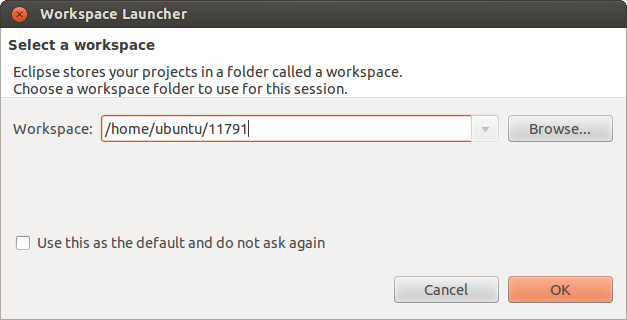
\includegraphics[scale=0.3]{eclipse-01-login}
\caption{Eclipse choose workspace\label{eclipse-01-login}}
\end{figure}

\item Use the default workspace path or create your own workspace, as shown in Figure \ref{eclipse-01-login}. And finally, we could see the Eclipse Welcome view at the end of workspace initialization. See Figure \ref{eclipse-02-welcome}.

\begin{figure}[t]
\centering
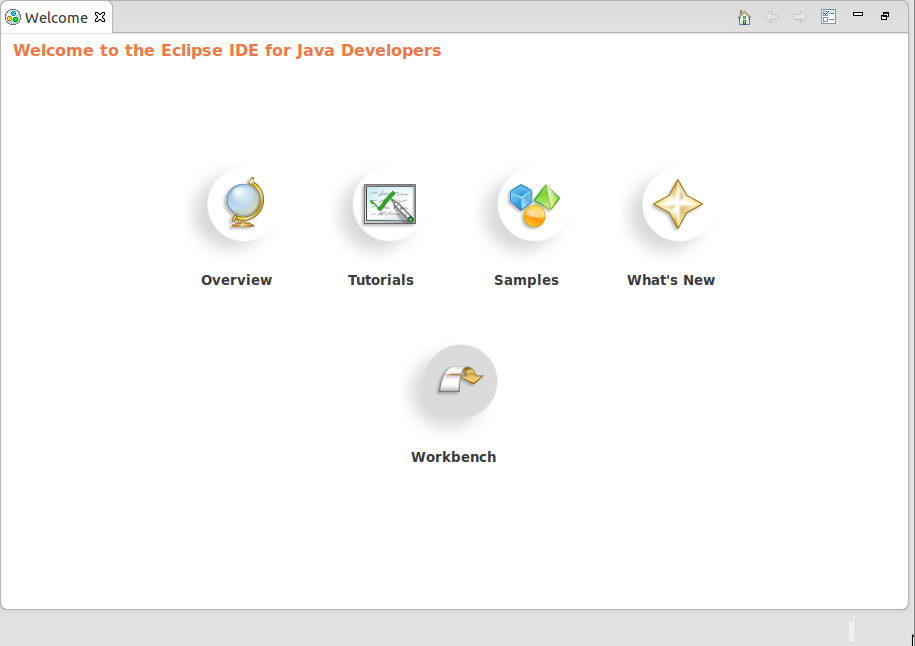
\includegraphics[scale=0.3]{eclipse-02-welcome}
\caption{Eclipse Welcome view\label{eclipse-02-welcome}}
\end{figure}

\end{enumerate}
